\chapter{Nodes and Packet Forwarding}
\label{chap:nodes}

This chapter describes one aspect of creating a topology in \ns,
\ie, creating the nodes.
In 
\href{the next chapter}{Chapter}{chap:links},
we will describe second aspect of creating the topology,
\ie, connecting the nodes to form links.
Recall that each simulation requires a single instance of the
\clsref{Simulator}{../ns-/ns-lib.tcl} to control and operate that simulation.
The class provides instance procedures to create and manage the topology,
and internally stores references to each element of the topology.
We begin 
\href{by describing the procedures in the class Simulator}{%
        Section}{sec:node:simulator}.
We then
\href{describe the instance procedures in the class Node}{%
        Section}{sec:node:node}
to access and operate on individual nodes.
We conclude
\href{with detailed descriptions of the Classifier}{%
        Section}{sec:node:classifiers}
from which the more complex node objects are formed.

The procedures and functions described in this chapter can be found in
\nsf{tcl/lib/ns-lib.tcl}, \nsf{tcl/lib/ns-nodes.tcl}, \\
\nsf{classifier.\{cc, h\}, \nsf{classifier-addr.cc},
\nsf{classifier-mcast.cc}, \nsf{classifier-mpath.cc}, 
and, \nsf{replicator.cc}.

\section{Simulator Methods: Creating the Topology}
\label{sec:node:simulator}

The basic primitive for acquiring a node is
\begin{program}
    set ns [new Simulator]
    $ns \fcnref{\textbf{node}}{../ns-2/ns-lib.tcl}{Simulator::node}
    $ns node
\end{program}
The instance procedure \code{node} constructs
a node out of more simple
\href{classifier objects}{Section}{sec:node:classifiers}.
The Node itself is a standalone class in OTcl.
However, most of the components of the node are themselves TclObjects.
The typical structure of a node is as shown in Figure~\ref{fig:node:unicast}.
\begin{figure}[tb]
  \centerline{\includegraphics{node}}
  \caption{Structure of an Unicast Node}
  \label{fig:node:unicast}
\end{figure}

The address of an agent in a node is 16 bits wide:
the higher 8 bits define the node \code{id_},
the lower 8 bits identify the individual agent at the node.
This limits the number of nodes in a simulation to 256 nodes.
If the user needs to create a topology larger than 256 nodes,
then they should first expand the address space before creating any
nodes, as
\begin{program}
        Node expandaddr
\end{program}
This expands the address space to 30 bits, the higher 22 of which are 
used to assign node numbers.

By default, nodes in \ns\ are constructed for unicast simulations.
In order to create nodes for multicast simulation, the
class variable, \code{EnableMcast_}, should be set to 1, as:
\begin{program}
        Simulator set EnableMcast_ 1
\end{program}
before any nodes are created.
The internal structure of a typical multicast node is shown in
Figure~\ref{sec:node:multicast}.
\begin{figure}
  \centerline{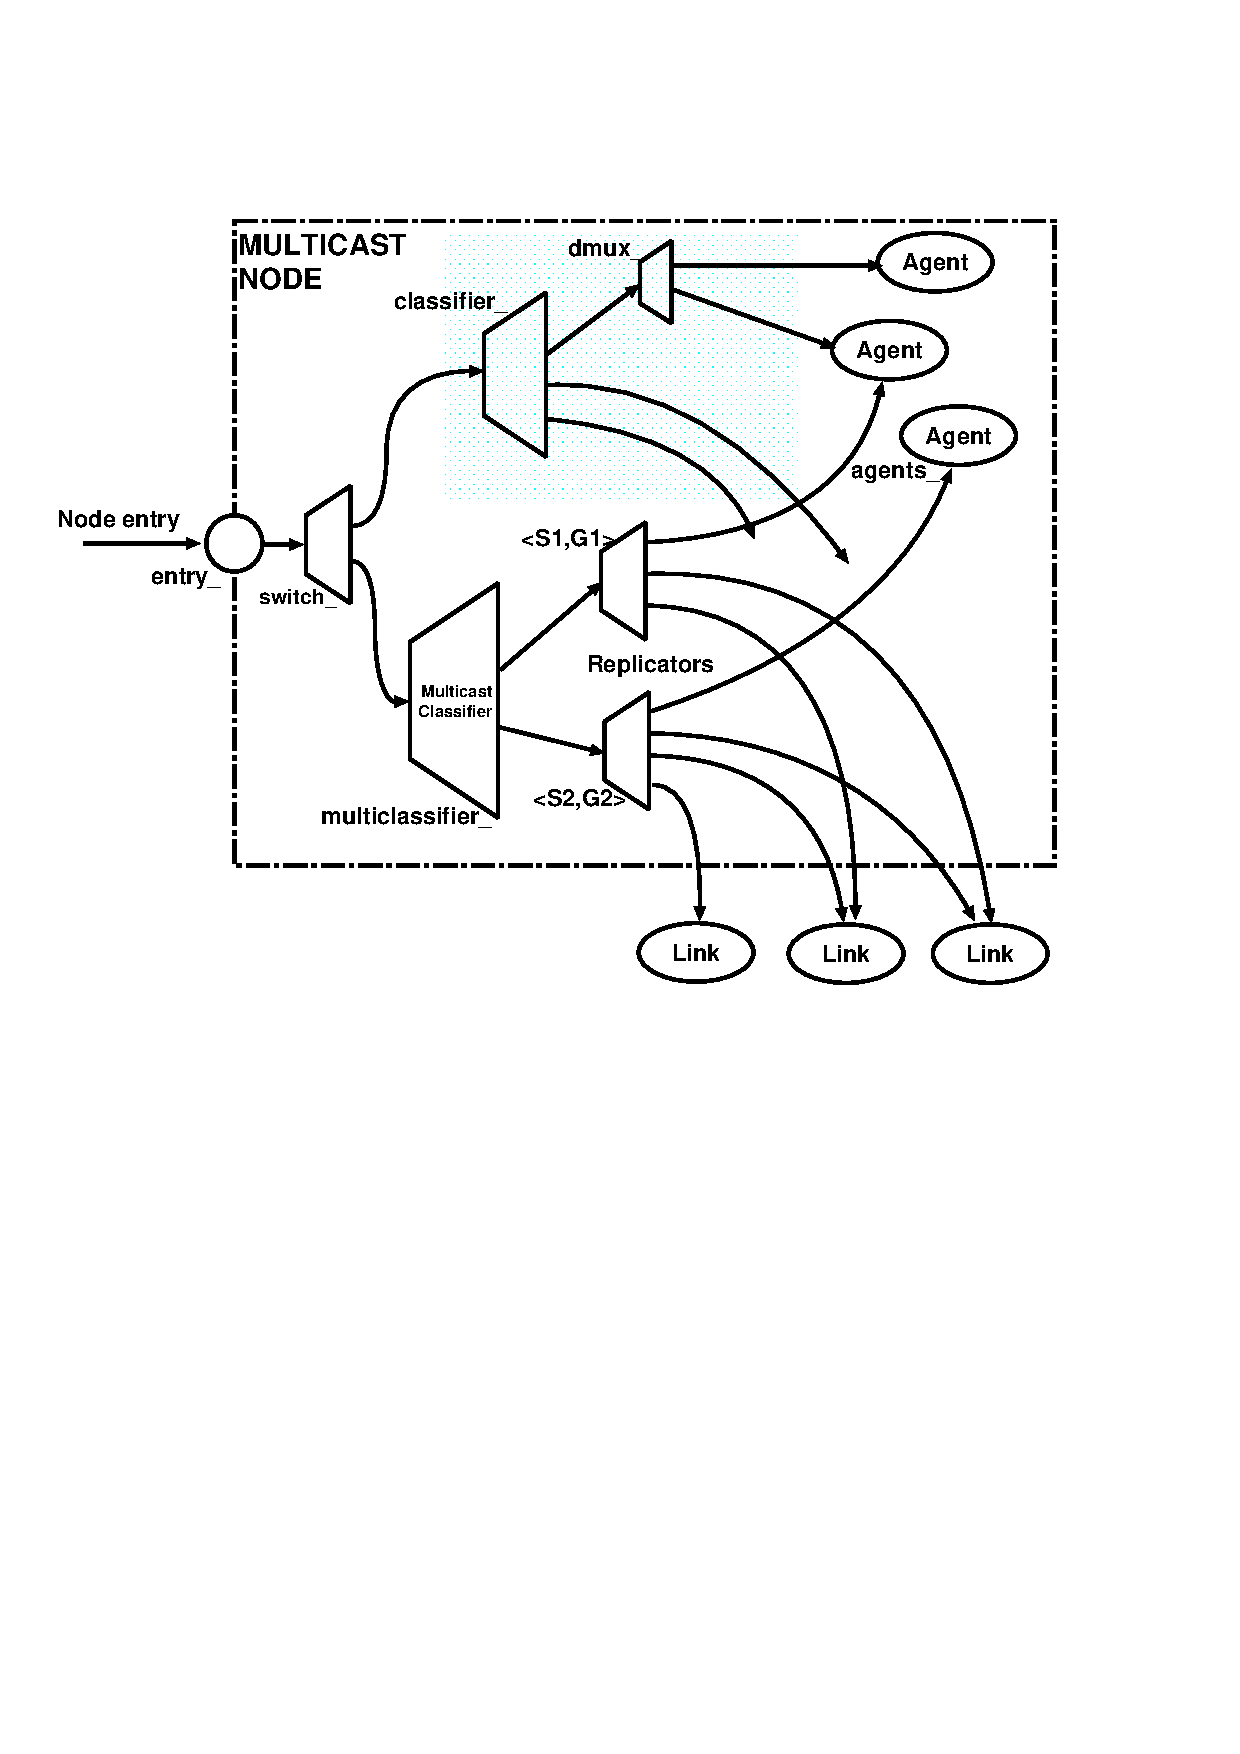
\includegraphics{mcastNode}}
  \caption{Internal Structure of a Multicast Node}
  \label{sec:node:multicast}
\end{figure}

When a simulation uses multicast routing,
the highest bit of the address indicates whether the particular
address is a multicast address or an unicast address.
If the bit is 0, the address represents a unicast address,
else the address represents a multicast address.
This implies that, by default, 
a multicast simulation is restricted to 128 nodes.

\section{Node Methods: Configuring the Node}
\label{sec:node:node}

Procedures to configure an individual node can be classified into:
\begin{list}{---}{\itemsep0pt}
\item Control functions
\item Address and Port number management, unicast routing functions
\item Agent management
\item Adding neighbours
\end{list}
We describe each of the functions in the following paragraphs.

\paragraph{Control functions}
\begin{enumerate}
\item \code{$node entry} returns the entry point for a node.
This is the first element which will handle packets arriving at that node.

The Node instance variable, \code{entry_}, stores the reference this element.
For unicast nodes, this is the address classifier that looks at the higher
bits of the destination address.
The instance variable, \code{classifier_} contains the reference to this
classifier.
However, for multicast nodes, the entry point is the
\code{switch_} which looks at the first bit to decide whether
it should forward the packet to the unicast classifier, or the multicast
classifier as appropriate.

\item \code{$node reset} will reset all agents at the node.

\item \code{$node enable-mcast} is an internal procedure used
  by the class simulator when creating a node.
  This procedure installs the additional classifiers needed
  to convert a unicast node to a multicast node.
\end{enumerate}


\paragraph{Address and Port number management}
The procedure \code{$node id} returns the node number of the node.
This number is automatically incremenetd and assigned to each node at
creation by the class Simulator method, \code{$ns node}.
The class Simulator also stores an instance variable array\footnote{%
  \ie, an instance variable of a class that is also an array variable},
  \code{Node_}, indexed by the node id, and contains a reference to the
  node with that id.

The procedure \code{$node agent \tup{port}} returns the handle of the
agent at the specified port.
If no agent at the specified port number is available, the procedure returns
the null string.

The procedure \code{alloc-port} returns the next available port number.
It uses an instance variable, \code{np_},
to track the next unallocated port number.

The procedures, \code{add-route} and \code{add-routes},
are used by \href{unicast routing}{Chapter}{chap:unicast}
to add routes to populate the \code{classifier_}
The usage syntax is
\code{$node add-route \tup{destination id} \tup{TclObject}};
\code{TclObject} is the entry of \code{dmux_}, the port demultiplexer
at the node, if the destination id is the same as this node's id,
it is often the head of a link to send packets for that destination to,
but could also be the the entry for other classifiers or types of classifiers.

\code{$node add-routes \tup{destination id} \tup{TclObjects}}
is used to add multiple routes to the same destination that must be used
simultaneously in round robin manner to spread the bandwidth used to reach
that destination across all links equally.
It is used only if the instance variable \code{multiPath_} is set to 1,
and detailed dynamic routing strategies are in effect,
and requires the use of a multiPath classifier.
We describe the implementation of the multiPath classifier
\href{later in this chapter}{Section}{sec:node:classifiers};
however, \href{we defer the discussion of multipath
routing}{Chapter}{chap:unicast} to the chapter on unicast routing.

The dual of \proc[]{add-routes} is \proc[]{delete-routes}.
It takes the id, a list of \code{TclObjects}, and a reference to
the simulator's \code{nullagent}.
It removes the TclObjects in the list from the installed routes in the
multipath classifier.
If the route entry in the classifier does not point to a multipath
classifier,
the routine simply clears the entry from \code{classifier_}, and
installs the \code{nullagent} in its place.

Detailed dynamic routing also uses two additional methods:
the instance procedure \proc[]{init-routing} sets the instance variable
\code{multiPath_} to be equal to the class variable of the same name.
It also adds a reference to the route controller object at that node
in the instance variable, \code{rtObject_}.
The procedure \proc[]{rtObject?} returns the handle for the route object 
at the node.

Finally, the procedure \proc[]{intf-changed} is invoked by
the network dynamics code if a link incident on the node
changes state.  Additional details on how this procedure
is used are discussed later
\href{in the chapter on network dynamics}{Chapter}{chap:net-dynamics}.

\paragraph{Agent management}
Given an \tup{agent}, the procedure \proc[]{attach} will
add the agent to its list of \code{agents_},
assign a port number the agent and set its source address,
set the target of the agent to be its (\ie, the node's) \proc[]{entry},
and add a pointer to the port demultiplexer at the node (\code{dmux_})
to the agent at the corresponding slot in the \code{dmux_} classifier.

Conversely, \proc[]{detach}will remove the agent from \code{agents_},
and point the agent's target, and the entry in the node \code{dmux_}
to \code{nullagent}.

\paragraph{Tracking Neighbours}
Each node keeps a list of its adjacent neighbours in its instance variable,
\code{neighbor_}.  The procedure \proc[]{add-neighbor} adds a neighbor to the list.  The procedure \proc[]{neighbors} returns this list.

\section{The Classifier}
\label{sec:node:classifiers}

The function of a node when it receives a packet is to examine
the packet's fields, usually its destination address, and
on occasion, its source address.
It should then map the values to an outgoing interface object
that is the next downstream recipient of this packet.

In \ns, this task is performed by a simple \emph{classifier} object.
Multiple classifier objects,
each looking at a specific portion of the packet
forward the packet through the node.
A node in \ns\ uses many different types of classifiers for different purposes.
This section describes some of the more common, or simpler,
classifier objects in \ns.

We begin with a description of the base class in this section.
The next subsections describe
\href{the address classifier}{Section}{sec:node:addr-classifier},
\href{the multicast classifier}{Section}{sec:node:mcast-classifier},
\href{the multipath classifier}{Section}{sec:node:mpath-classifier}, and
finally, \href{the replicator}{Section}{sec:node:replicator}.

A classifier provides a way to match a packet against some
logical criteria and retrieve a reference to another simulation
object based on the match results.
Each classifier contains a table of simulation objects indexed
by {\em slot number}.
The job of a classifier is to determine the slot number associated
with a received packet and forward that packet to the
object referenced by that particular slot.
The C++ \clsref{Classifier}{../ns-2/classifier.h}
(defined in \nsf{classifier.h})
provides a base class from which other classifiers are derived.
\begin{program}
        class Classifier : public NsObject \{
        public:
                ~Classifier();
                void recv(Packet*, Handler* h = 0);
         protected:
                Classifier();
                void install(int slot, NsObject*);
                void clear(int slot);
                virtual int command(int argc, const char*const* argv);
                virtual int classify(Packet *const) = 0;
                void alloc(int);
                NsObject** slot_;       \* table that maps slot number to a NsObject */
                int nslot_;
                int maxslot_;
        \};
\end{program}
The \fcn[]{classify} method is pure virtual, indicating the
class \code{Classifier} is to be used only as a base class.
The \fcn[]{alloc} method dynamically allocates enough space
in the table to hold the specified number of slots.
The \fcn[]{install} and \fcn[]{clear} methods
add or remove objects from the table.
The \fcn[]{recv} method and the OTcl interface are implemented
as follows in \nsf{classifier.cc}:
\begin{program}
        /*
         *{\cf objects only ever see "packet" events, which come either}
         *{\cf from an incoming link or a local agent (i.e., packet source).}
         */
        void Classifier::recv(Packet* p, Handler*)
        \{
                NsObject* node;
                int cl = classify(p);
                if (cl < 0 || cl >= nslot_ || (node = slot_[cl]) == 0) \{
                        Tcl::instance().evalf("%s no-slot %d", name(), cl);
                        Packet::free(p);
                        return;
                \}
                node->recv(p);
        \}

        int Classifier::command(int argc, const char*const* argv)
        \{
                Tcl& tcl = Tcl::instance();
                if (argc == 3) \{
                        /*
                         * $classifier clear $slot
                         */
                        if (strcmp(argv[1], "clear") == 0) \{
                                int slot = atoi(argv[2]);
                                clear(slot);
                                return (TCL_OK);
                        \}
                        /*
                         * $classifier installNext $node
                         */
                        if (strcmp(argv[1], "installNext") == 0) \{
                                int slot = maxslot_ + 1;
                                NsObject* node = (NsObject*)TclObject::lookup(argv[2]);
                                install(slot, node);
                                tcl.resultf("%u", slot);
                                return TCL_OK;
                        \}
                        if (strcmp(argv[1], "slot") == 0) \{
                                int slot = atoi(argv[2]);
                                if ((slot >= 0) || (slot < nslot_)) \{
                                        tcl.resultf("%s", slot_[slot]->name());
                                        return TCL_OK;
                                \}
                                tcl.resultf("Classifier: no object at slot %d", slot);
                                return (TCL_ERROR);
                        \}
                \} else if (argc == 4) \{
                        /*
                         * $classifier install $slot $node
                         */
                        if (strcmp(argv[1], "install") == 0) \{
                                int slot = atoi(argv[2]);
                                NsObject* node = (NsObject*)TclObject::lookup(argv[3]);
                                install(slot, node);
                                return (TCL_OK);
                        \}
                \}
                return (NsObject::command(argc, argv));
        \}
\end{program}
When a classifier \fcn[]{recv}'s a packet,
it hands it to the \fcn[]{classify} method.
This is defined differently in each type of classifier
derived from the base class.
The usual format is for the \fcn[]{classify} method to
determine and return a slot index into the table of slots.
If the index is valid, and points to a valid TclObject,
the classifier will hand the packet to that object using 
that object's \fcn[]{recv} method.
If the index is not valid, the classifier will invoke
the instance procedure \proc[]{no-slot} to attempt to 
populate the table correctly.
However, in the base class \proc[]{Classifier::no-slot} prints
and error message and terminates execution.

The \fcnref{\fcn[]{command} method}{../ns-2/classifier.cc}{Classifier::command}
provides the following instproc-likes to the interpreter:
\begin{itemize}\itemsep0pt
\item \proc[\tup{slot}]{clear} clears the entry in a particular slot.
\item \proc[\tup{object}]{installNext} installs the object
        in the next available slot, and returns the slot number.

        Note that this instproc-like is 
        \fcnref{overloaded by an instance procedure of the same name}{%
                ../ns-2/ns-lib.tcl}{Classifier::installNext}
        that stores a reference to the object stored.
        This then helps quick query of the objects
        installed in the classifier from OTcl.
\item \proc[\tup{index}]{slot} returns the object stored in the specified slot.
\item \proc[\tup{index}, \tup{object}]{install} installs the specified
        \tup{object} at the slot \tup{index}.

        Note that this instproc-like too is 
        \fcnref{overloaded by an instance procedure of the same name}{%
                ../ns-2/ns-lib.tcl}{Classifier::install}
        that stores a reference to the object stored.
        This is also to quickly query of the objects
        installed in the classifier from OTcl.
\end{itemize}

\subsection{Address Classifiers}
\label{sec:node:addr-classifier}

An address classifier is used in supporting unicast packet forwarding.
It applies a bitwise shift and mask operation to a packet's destination
address to produce a slot number.
The slot number is returned from the \fcn[]{classify} method.
The \clsref{AddressClassifier}{../ns-2/classifier-addr.cc}
(defined in \nsf{classifier-addr.cc}) ide defined as follows:
\begin{program}
        class AddressClassifier : public Classifier \{
        public:
                AddressClassifier() : mask_(~0), shift_(0) \{
                        bind("mask_", (int*)&mask_);
                        bind("shift_", &shift_);
                \}
        protected:
                int classify(Packet *const p) \{
                        IPHeader *h = IPHeader::access(p->bits());
                        return ((h->dst() >> shift_) & mask_);
                \}
                nsaddr_t mask_;
                int shift_;
        \};
\end{program}
The class imposes no direct semantic meaning
on a packet's destination address field.
Rather, it returns some number of bits from the packet's
\code{dst_} field as the slot number used
in the \fcnref{\fcn[]{Classifier::recv}}{../ns-2/classifier.cc}{Classifier::recv} method.
The \code{mask_} and \code{shift_} values are set through OTcl.

\subsection{Multicast Classifiers}{
\label{sec:node:mcast-classifier}

The multicast classifier classifies packets
according to both source and destination (group) addresses.
It maintains a (chained hash) table mapping source/group pairs to slot numbers.
When a packet arrives containing a source/group unknown to the classifier,
it invokes an Otcl procedure \proc[]{Node::new-group}
to add an entry to its table.
This OTcl procedure may use the method \code{set-hash} to add
new (source, group, slot) 3-tuples to the classifier's table.
The multicast classifier is defined in \nsf{classifier-mcast.cc}
as follows:
\begin{program}
        static class MCastClassifierClass : public TclClass \{
        public:
                MCastClassifierClass() : TclClass("Classifier/Multicast") \{\}
                TclObject* create(int argc, const char*const* argv) \{
                        return (new MCastClassifier());
                \}
        \} class_mcast_classifier;

        class MCastClassifier : public Classifier \{
        public:
                MCastClassifier();
                ~MCastClassifier();
        protected:
                int command(int argc, const char*const* argv);
                int classify(Packet *const p);
                int findslot();
                void set_hash(nsaddr_t src, nsaddr_t dst, int slot);
                int hash(nsaddr_t src, nsaddr_t dst) const \{
                        u_int32_t s = src ^ dst;
                        s ^= s >> 16;
                        s ^= s >> 8;
                        return (s & 0xff);
                \}
                struct hashnode \{
                        int slot;
                        nsaddr_t src;
                        nsaddr_t dst;
                        hashnode* next;
                \};
                hashnode* ht_[256];
                const hashnode* lookup(nsaddr_t src, nsaddr_t dst) const;
        \};

        int MCastClassifier::classify(Packet *const pkt)
        \{
                IPHeader *h = IPHeader::access(pkt->bits());
                nsaddr_t src = h->src() >> 8; /*XXX*/
                nsaddr_t dst = h->dst();
                const hashnode* p = lookup(src, dst);
                if (p == 0) \{
                        /*
                         * Didn't find an entry.
                         * Call tcl exactly once to install one.
                         * If tcl doesn't come through then fail.
                         */
                        Tcl::instance().evalf("%s new-group %u %u", name(), src, dst);
                        p = lookup(src, dst);
                        if (p == 0)
                                return (-1);
                \}
                return (p->slot);
        \}
\end{program}
The \clsref{MCastClassifier}  implements a chained hash table
and applies a hash function on both the packet source and
destination addresses.
The hash function returns the slot number
to index the \code{slot_} table in the underlying object.
A hash miss implies packet delivery to a previously-unknown group;
OTcl is called to handle the situation.
The OTcl code is expected to insert an appropriate entry into the hash table.

\subsection{MultiPath Classifier}
\label{sec:node:mpath-classifier}

This object is devised to support equal cost multipath
forwarding, where the node has multiple equal cost routes
to the same destination, and would like to use all of them
simultaneously.
This object does not look at any field in the packet.
With every succeeding packet, 
it simply returns the next filled slot in round robin fashion.
The definitions for this classifier are in \nsf{classifier-mpath.cc},
and are shown below:
\begin{program}
class MultiPathForwarder : public Classifier \{
public:
        MultiPathForwarder() : ns_(0), Classifier() \{\} 
        virtual int classify(Packet* const) \{
                int cl;
                int fail = ns_;
                do \{
                        cl = ns_++;
                        ns_ %= (maxslot_ + 1);
                \} while (slot_[cl] == 0 && ns_ != fail);
                return cl;
        \}
private:
        int ns_;     \* next slot to be used.  Probably a misnomer? */
\};
\end{program}

\subsection{Replicator}
\label{sec:node:replicator}

The replicator is different from the other classifiers
we have described earlier,
in that it does not use the classify function.
Rather, it simply uses the classifier as a table of $n$ slots;
it overloads the \fcn[]{recv} method to produce $n$ copies
of a packet, that are delivered to all $n$ objects referenced in the table.

To support multicast packet forwarding, a classifier receiving a
multicast packet from source $S$
destined for group $G$ computes a hash function $h(S,G)$ giving
a ``slot number'' in the classifier's object table.
Thus, the maximum size of the table is $O(|S|\times|G|)$.
In multicast delivery, the packet must be copied once for
each link leading to nodes subscribed to $G$ minus one.
Production of additional copies of the packet is performed
by a \code{Replicator} class, defined in \code{replicator.cc}:
\begin{program}
        /*
         * {\cf A replicator is not really a packet classifier but}
         * {\cf we simply find convenience in leveraging its slot table.}
         * {\cf (this object used to implement fan-out on a multicast}
         * {\cf router as well as broadcast LANs)}
         */
        class Replicator : public Classifier \{
        public:
                Replicator();
                void recv(Packet*, Handler* h = 0);
                virtual int classify(Packet* const) \{\};
        protected:
                int ignore_;
        \};

        void Replicator::recv(Packet* p, Handler*)
        \{
                IPHeader *iph = IPHeader::access(p->bits());
                if (maxslot_ < 0) \{
                        if (!ignore_)
                                Tcl::instance().evalf("%s drop %u %u", name(), 
                                        iph->src(), iph->dst());
                        Packet::free(p);
                        return;
                \}
                for (int i = 0; i < maxslot_; ++i) \{
                        NsObject* o = slot_[i];
                        if (o != 0)
                                o->recv(p->copy());
                \}
                /* {\cf we know that maxslot is non-null} */
                slot_[maxslot_]->recv(p);
        \}
\end{program}
As we can see from the code,
this class  does not really classify packets.
Rather, it replicates a packet, one for each entry in its table,
and delivers the copies to each of the nodes listed in the table.
The last entry in the table gets the ``original'' packet.
Since the \fcn[]{classify} method is pure virtual in the base class,
the replicator defines an empty \fcn[]{classify} method.

\endinput
